\documentclass[
	onesided,
	12pt
]{article}

\usepackage[british]{babel}
\usepackage{csquotes}
\usepackage[style=apa]{biblatex}
\DeclareLanguageMapping{british}{british-apa}
\addbibresource{literature.bib}

\usepackage{tikz}
\usepackage{tikz,fullpage}
\usetikzlibrary{arrows,%
                petri,%
                topaths}%
\usepackage{tkz-berge}
\usepackage[activate]{microtype}
\usepackage[utf8]{inputenc}
\usepackage[T1]{fontenc}
\usepackage[onehalfspacing]{setspace}

\usepackage[position=top]{subfig}
\usepackage{nameref}
\usepackage{listings}
\usepackage{epstopdf}
\lstset{
	numbers=left,            % Zeilennummern links
	stepnumber=1,            % Jede Zeile nummerieren.
	numbersep=5pt,           % 5pt Abstand zum Quellcode
	numberstyle=\tiny,       % Zeichengrösse 'tiny' für die Nummern.
	breaklines=true,         % Zeilen umbrechen wenn notwendig.
	breakautoindent=true,    % Nach dem Zeilenumbruch Zeile einrücken.
	postbreak=\space,        % Bei Leerzeichen umbrechen.
	tabsize=2,               % Tabulatorgrösse 2
	basicstyle=\ttfamily\footnotesize, % Nichtproportionale Schrift, klein für den Quellcode
	showspaces=false,        % Leerzeichen nicht anzeigen.
	showstringspaces=false,  % Leerzeichen auch in Strings ('') nicht anzeigen.
	extendedchars=true,      % Alle Zeichen vom Latin1 Zeichensatz anzeigen.
	captionpos=b,            % sets the caption-position to bottom
	backgroundcolor=\color{ListingBackground}, % Hintergrundfarbe des Quellcodes setzen.
	commentstyle=\color{ListingComment},
	stringstyle=\textit{}\color{ListingString},
	keywordstyle=\textbf{}\color{blue}
}
\usepackage{color}
\definecolor{LinkColor}{rgb}{0,0,0.2}
\definecolor{ListingBackground}{rgb}{0.95,0.95,0.95}
\definecolor{ListingString}{rgb}{0,0.6,0}
\definecolor{ListingComment}{rgb}{0.40,0.40,0.40}

\lstdefinelanguage{Cypher}
{
	alsoletter={<, :, >, /},
	morekeywords={MATCH, WHERE, RETURN, CREATE},
	morestring=[b]"
}



\title{Neo4j Graph Database}
\author{
	Nico-Alexei Hein, Lucas Thielmann, Andreas Rau \& Lisa Mischer
}
\date{\today}



\begin{document}

\maketitle


\begin{abstract}
This is a short explanation of Neo4j internals. This article gives some advice on how to work with Neo4j, including modeling and Business Intelligence.
\end{abstract}

\newpage

%!TEX root = ../neo4j.tex

\section{Introduction}
Neo4j is a transactional and graph based database. It was first released in 2010. Neo4j is written in Java and available under two different licences. 


\subsection{Neo4j DB}
Neo4j has its own query language which is called Cypher. Cypher concentrates on pattern search. It is similar to SQL, both are descriptive languages. Cypher can be used in the command line, but all properties about transaction behaviour are also valid for transactions executed by a terminal or a program. \nocite{neo4jman:2011}\\
Queries are run in a transaction. Either there exists already a transaction or one is created. It is possible to commit several queries to one transaction. "A transaction will either fully succeed, or not succeed at all" \cite{}. Changes of a query are held in memory until the hole query has finished executing. This needs a lot of heap space and therefore it is important to structure queries. Neo4j supports the ACID properties - atomicity, consistency, isolation and durability. In case of a failure of a transaction a roll back is done. Neo4j offers several options for managing locking of resources. On the one hand there is a default locking behaviour, on the other hand tools are given to archive a higher level of isolation for transactions. Additionally, it uses deadlock detection algorithms.\\
Neo4j databases are accessible via a Java API and therefore can be embedded in Java applications. It also supports batch processing for large amounts of data.

\subsection{Example}
As an example we modelled  the relation between books, authors and publishers. Authors write books and publishers publish books. To start working with the database, Neo4j has to be run from the command line or terminal. After the server did start, a graphical user interface can be accessed through a browser. This graphical user interface has its own command line in which Cypher statements are executed.\\
Figure \ref{example-graph} shows how our example looks in Neo4j. This picture is given by Neo4j in the browser view.

\begin{figure}
	\centering
		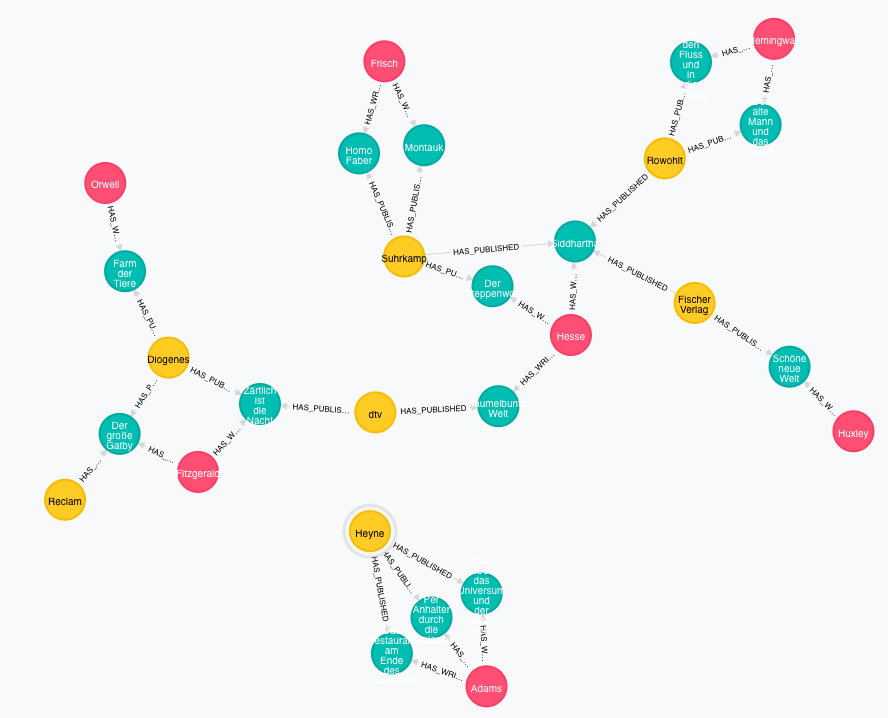
\includegraphics[width=\linewidth]{images/Neo4j_Graph.png}
	\caption{Example Graph}
	\label{example-graph}
\end{figure}

\subsection{Queries}
Neo4j offers a lot of possibilities for queries. In this section, some query examples are given in Cypher syntax for the example graph.\\
The syntax of Cypher statements are similar to SQL statements. Listing \ref{Cypher-Syntax} shows the basic structure  of a statement.
 
\begin{lstlisting}[language={Cypher}, caption={Cypher Syntax}, label={Cypher-Syntax}]
MATCH <pattern> WHERE <conditions> RETURN <expressions>
\end{lstlisting}

\paragraph{CREATE}
The CREATE statement can be used to create new nodes as well as create relations between notes. Listing \ref{create_node} shows how to create the author Fitzgerald. The CREATE statement is started with parenthesis to indicate a node. The first information given to the CREATE statement is the ID of the node, followed by a colon and a lable given to the node. In this case the ID is fscottfitzgerald and the label for the node is Author. All properties follow in braces. The node here has three attributes: name, first-name and stage-name.

\begin{lstlisting}[language={Cypher}, caption={Create Node}, label={create_node}]
CREATE (fScottFitzgerald:Author { name : 'Fitzgerald', firstname : 'Francis Scott Key', stagename : 'F. Scott Fitzgerald'})
\end{lstlisting}

The statement for creation of a relation looks a bit different. Listing \ref{create_relation} shows an example where the relation between Fitzgerald and his book is made. The node ID from which the relations starts is put in parenthesis at the beginning. Then the kind of relation is defined with brackets. Beginning with a colon the relationship type is defined, followed by all properties in braces. After the relationship information are finished an arrow points to the end node, again defined by the node ID in parenthesis. To use the ID to identify a node is only possible if the node is created in the same transaction as the relation. Otherwise the node has to be found via the MATCH statement. On the other hand, if one ore two nodes do not exist when create relation statement is executed, this nodes will be created automatically. 

\begin{lstlisting}[language={Cypher}, caption={Create Relation}, label={create_relation}]
CREATE (fScottFitzgerald)-[:HAS_WRITTEN { year : '1925'}]->(derGrosseGatsby)
\end{lstlisting}

\paragraph{MATCH}
MATCH is used to find nodes. The simplest MATCH statement is shown in listing \ref{simple_match}. This statement returns everything in the graph. E.G. this statement was used to extract figure \ref{example-graph}, an image of the graph which is shown above. Furthermore it is used for nearly every operation in the graph. One can find nodes of a special type, nodes or relations with a certain property or just certain information. If an item is found the statement can be extended, e.g. to add a CREATE statement or add a new property. Listing \ref{relation_match} is an examples which shows how to create a new relation between two existing nodes. This statement sets Heyne as the publisher of Homo Faber.

\begin{lstlisting}[language={Cypher}, caption={Simplest Match Statement}, label={simple_match}]
MATCH n RETURN n
\end{lstlisting}

\begin{lstlisting}[language={Cypher}, caption={Match and Create Relation}, label={relation_match}]
MATCH (bb:Book), (vv:Publisher) WHERE bb.title = "Homo Faber" AND vv.name = "Heyne" CREATE (vv)-[r:HAS_PUBLISHED]->(bb) RETURN r
\end{lstlisting}

Neo4j offers the possibility to solve a graph. It provides statements to find the shortest path through a graph (also possible for sub-graphs) or select the surrounding of a node with a certain radius. These statements are on the basis of the MATCH statement too.

\paragraph{DELETE}
In Neo4j it is only possible to delete the graph. This means, all nodes and relations are deleted, but all labels will remain. These can only be delete if the whole database is deleted. The DELETE statement also uses the MATCH statement as a basis. First, all nodes and all relations of these nodes are selected. It is important that a node which is to be deleted has no relations any more. It is not necessary to first to delete all relations and divide the operation in two transactions. With OPTIONAL MATCH this is done automatically by Neo4j. The DELETE statement takes every selected item and deletes it.

\begin{lstlisting}[language={Cypher}, caption={Delete Graph}, label={delete}]
MATCH (vv:Publisher), (aa:Author), (bb:Book) OPTIONAL MATCH (vv)-[hp]-(), (aa)-[hw]-() DELETE aa, vv, bb, hp, hw
\end{lstlisting}
\newpage
\section{Data Modeling - Describing a Domain}
Data models in Neo4j are not enforced strictly. Instead the designer has to ensure a consistent database by only adding data that conforms to the desired model. The following paragraphs will describe step by step how such a model can be created.

\subsection{Nodes}
The process starts with identifying all nodes that exist in your domain. A node is any unique physical or abstract object that is important in the context of the domain.

Examples:
\begin{itemize}
	\item theGreatGatsby
	\item fScottFitzgerald
	\item reclam
\end{itemize}

\subsection{Labels}
In the next step, all labels of the domain have to be identified. Labels assign a specific role to a node. Nodes that have the same label are grouped into a set. These sets can later be used to write more efficient queries by only considering small subsets of a graph.

Examples:
\begin{tabular}{ | l | l | }
  \hline
  \textbf{Label} & \textbf{Node} \\
  \hline
  Book & theGreatGatsby \\
  \hline
  Author & fScottFitzgerald \\
  \hline
  Publisher & reclam \\
  \hline
\end{tabular}

\subsection{Relationships}
To transform the collection of labeled nodes into a graph, the next step identifies the relationships between the nodes. A relationship is a directed arc from one node to another. This relationship has an identifier that can later be used to query connected nodes.
	
Examples:
\begin{tabular}{ | l | l | l | }
  \hline
  \textbf{relationship identifier} & \textbf{From Node} & \textbf{To Node} \\
  \hline
  HAS\_WRITTEN & fScottFitzgerald & theGreatGatsby \\
  \hline
  HAS\_PUBLISHED & reclam & theGreatGatsby \\
  \hline
\end{tabular}
	
\subsection{Data}
In the last step, the graph is populated with additional properties. Data can be attached to nodes as well as relationships. These properties are often the information that provide the end result of a query. They can also be used to narrow down result sets and filter for appropriate results.

Examples:
\begin{tabular}{ | l | l | }
  \hline
  \textbf{Property} & \textbf{Node/Relationship} \\
  \hline
  title:"The Great Gatsby" & theGreatGatsby \\
  \hline
  firstname:"Francis Scott Key" & fScottFitzgerald \\
  \hline
  name:"Reclam" & reclam \\
  \hline
  year:"1925" & HAS\_WRITTEN \\
  \hline
\end{tabular}
\newpage
%!TEX root = ../neo4j.tex

\section{Storage Structure}

\subsection{Graph representation of the Data}
The simple sample graph displayed in figure \ref{fig1} shows a subgraph of the Neo4j example.
This human readable representation is now used to explain how Neo4j stores this graph. \nocite{storage1} \nocite{storage2}

\begin{figure}
	\centering
 	 	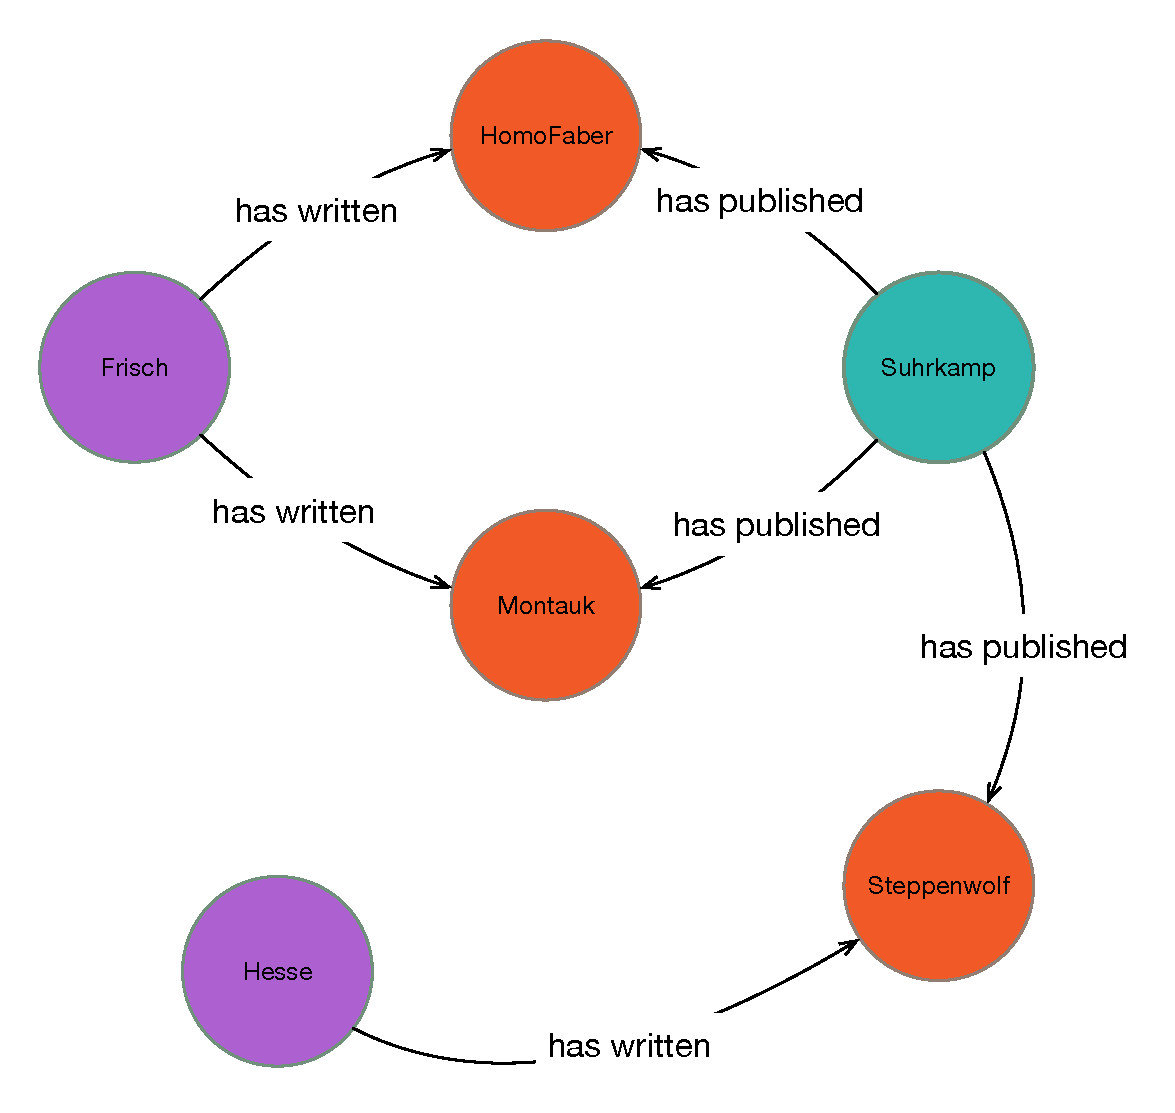
\includegraphics[width=0.9\textwidth]{images/theGraph.eps}
	\caption{Simple sample Graph}
	\label{fig1}
\end{figure}

\subsection{Property Records}
As a first step we take a look at the data stored in this graph. In Neo4j it is possible to store properties for every node and relationship (labels are ignored at the moment). To store the nodes and relationships itself in fixed size records (for faster access etc.) linked lists are used.
In figure \ref{fig2} the property records are displayed.

Every node and every relationship references its first property record. The property records themselves can be seen as a double linked list with a key - value store. In figure \ref{fig8} the representation on byte-level is shown. Node, relationship and property records are storing pointer to the next property in the last 4 bytes (one integer in Java). Bytes 18 to 21 of property record are containing a pointer to the previous record.


\begin{figure}
	\centering
 	 	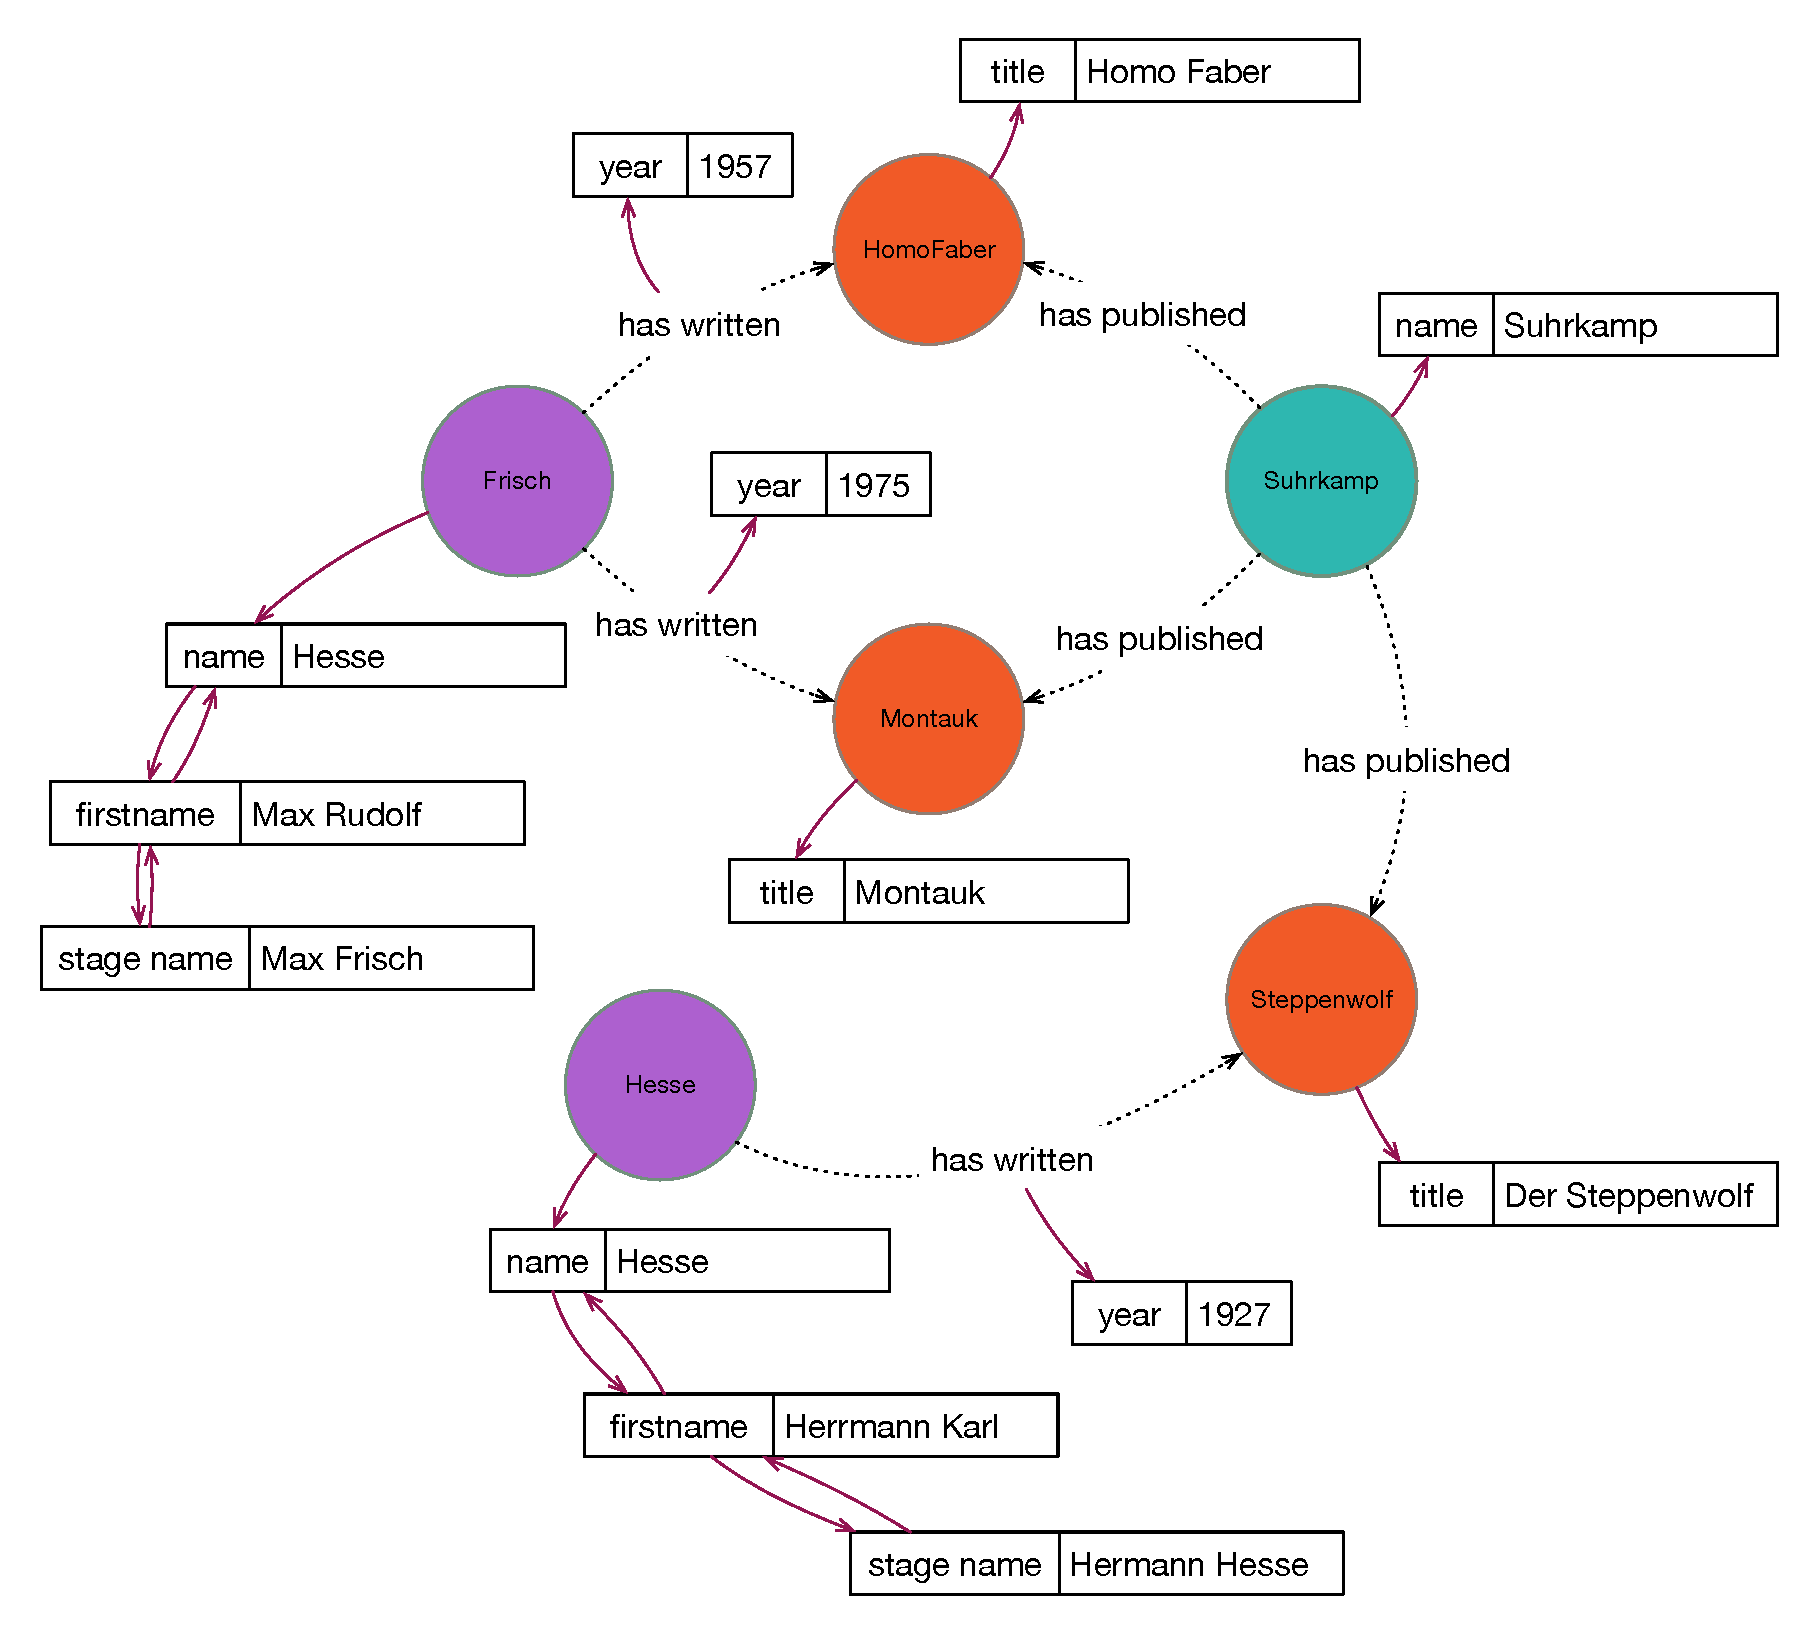
\includegraphics[width=0.9\textwidth]{images/nextProperty.eps}
	\caption{Property Records}
	\label{fig2}
\end{figure}

\subsection{Node Records}
The nodes itself as well as relationships are stored in fixed size records. However a node needs to know all relationships it is involved in. Therefor again a linked list is used. Every node references its first relationship shown in figure \ref{fig3} and in figure \ref{fig8} the deep blue marked bytes.
Now the complete node recored was covered and before we are focusing on the double linked relationship lists the relationship record is explained.

\begin{figure}[h]
	\centering
 	 	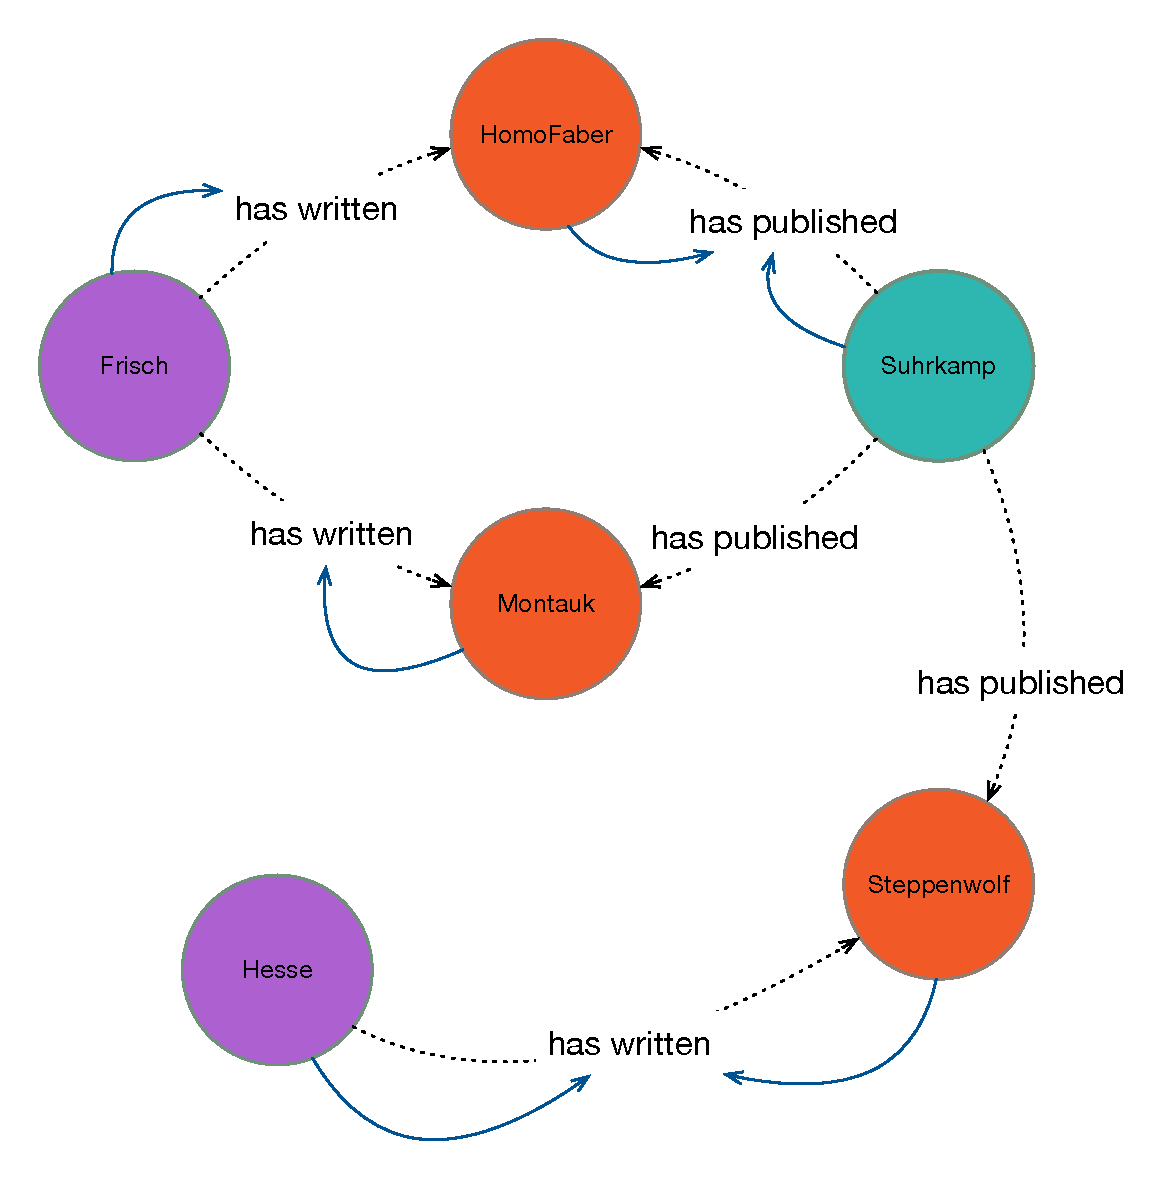
\includegraphics[width=0.9\textwidth]{images/nextRelationship.eps}
	\caption{First Relationship}
	\label{fig3}
\end{figure}

\subsection{Relationship Records}
As could have been observed above the node record only stores a pointer to a property and a relationship but not the first adjacent. Therefore we change our perspective to the graph and are focusing on relationships.
Instead of nodes referencing adjacent nodes we have nodes referencing the first relationship which references the start-node and the end-node of the relationship (Grey filled bytes in figure \ref{fig8}). This results in the abstract graph shown in figure \ref{fig4}.

The relationship type (Blue in figure \ref{fig4}) references a relationship type which again references a string (with the name) in the dynamic store. (This avoids redundancy in storage - the cache works in a different way.) 

The four green integers of the relationship record (figure \ref{fig8}) are used to realize the mentioned double linked relationship lists.
\begin{figure}
	\centering
 	 	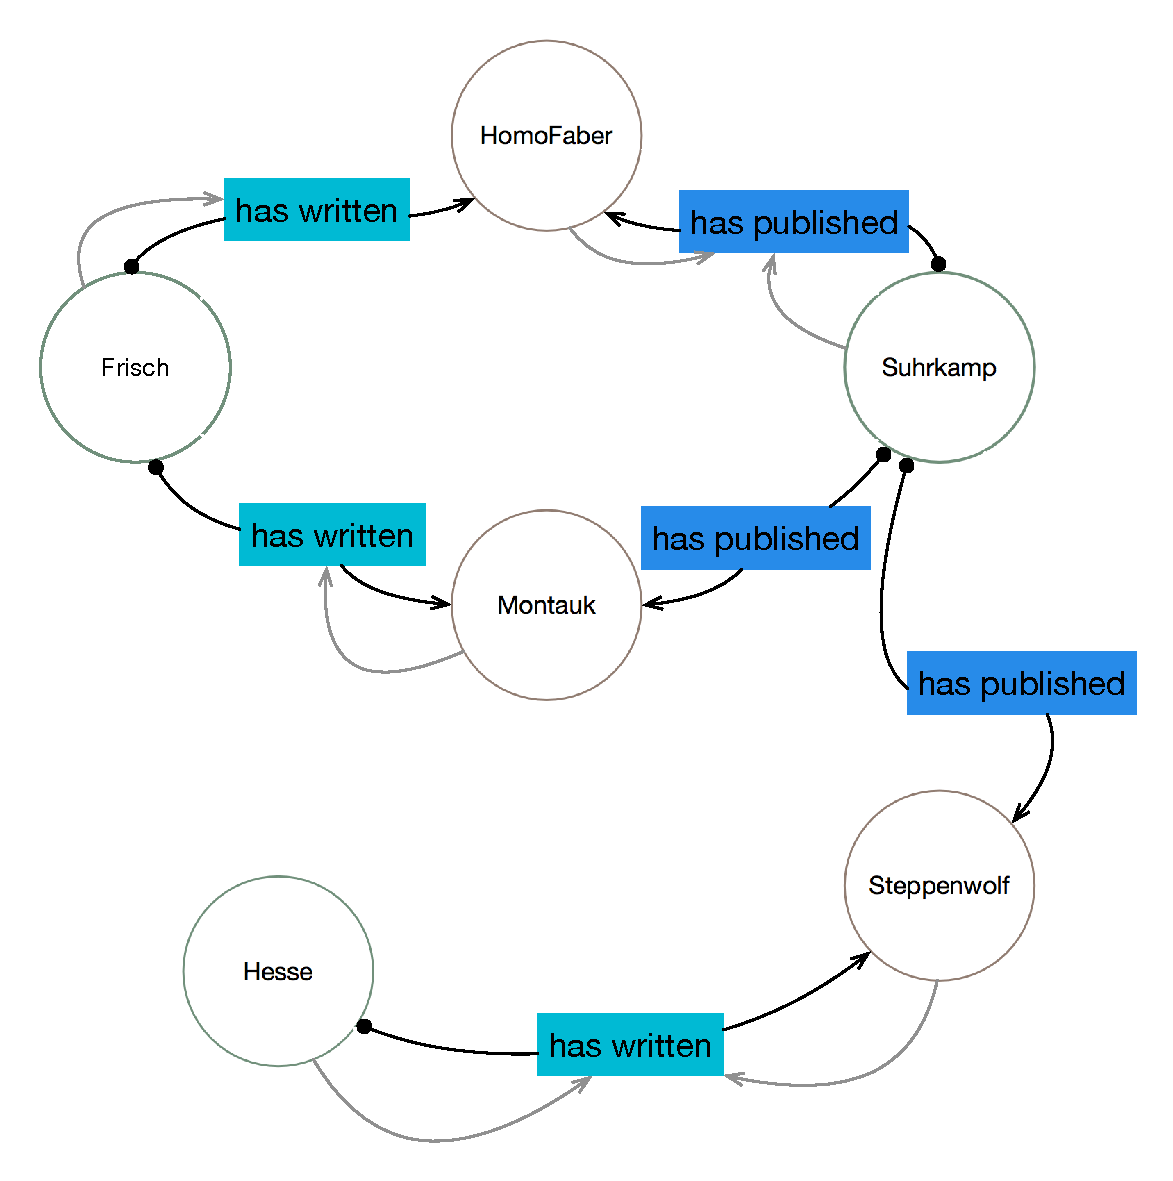
\includegraphics[width=0.9\textwidth]{images/startEnd.eps}
	\caption{Start Node - End Node}
	\label{fig4}
\end{figure}

Since every relationship is involved into two double linked lists (the one of the start-node and the one of the end-node) four pointers need to be stored.
In figure \ref{fig4}. They are shown as:

\begin{itemize}
	\item \textbf{SP} Start-Node Previous Relationship
	\item \textbf{EP} End-Node Previous Relationship
	\item \textbf{SN} Start-Node Next Relationship
	\item \textbf{EN} End-Node Next Relationship
\end{itemize}

In figure \ref{fig5} only the SP is set. In the following list some pointers are explained:
\begin{itemize}
	\item 'Frisch - has written - HomoFaber' has no pevious relationship since Frisch references it as its first relationship.
	\item 'Frisch - has written - Montauk' has 'Frisch - has written - HomoFaber' as previous relationship.
	\item 'Suhrkamp - has published - Steppenwolf' has 'Suhrkamp - has published - Montauk' which has  'Suhrkamp - has published - HomoFaver' which has no previous relationship.
	\item \dots
\end{itemize}

\begin{figure}
	\centering
 	 	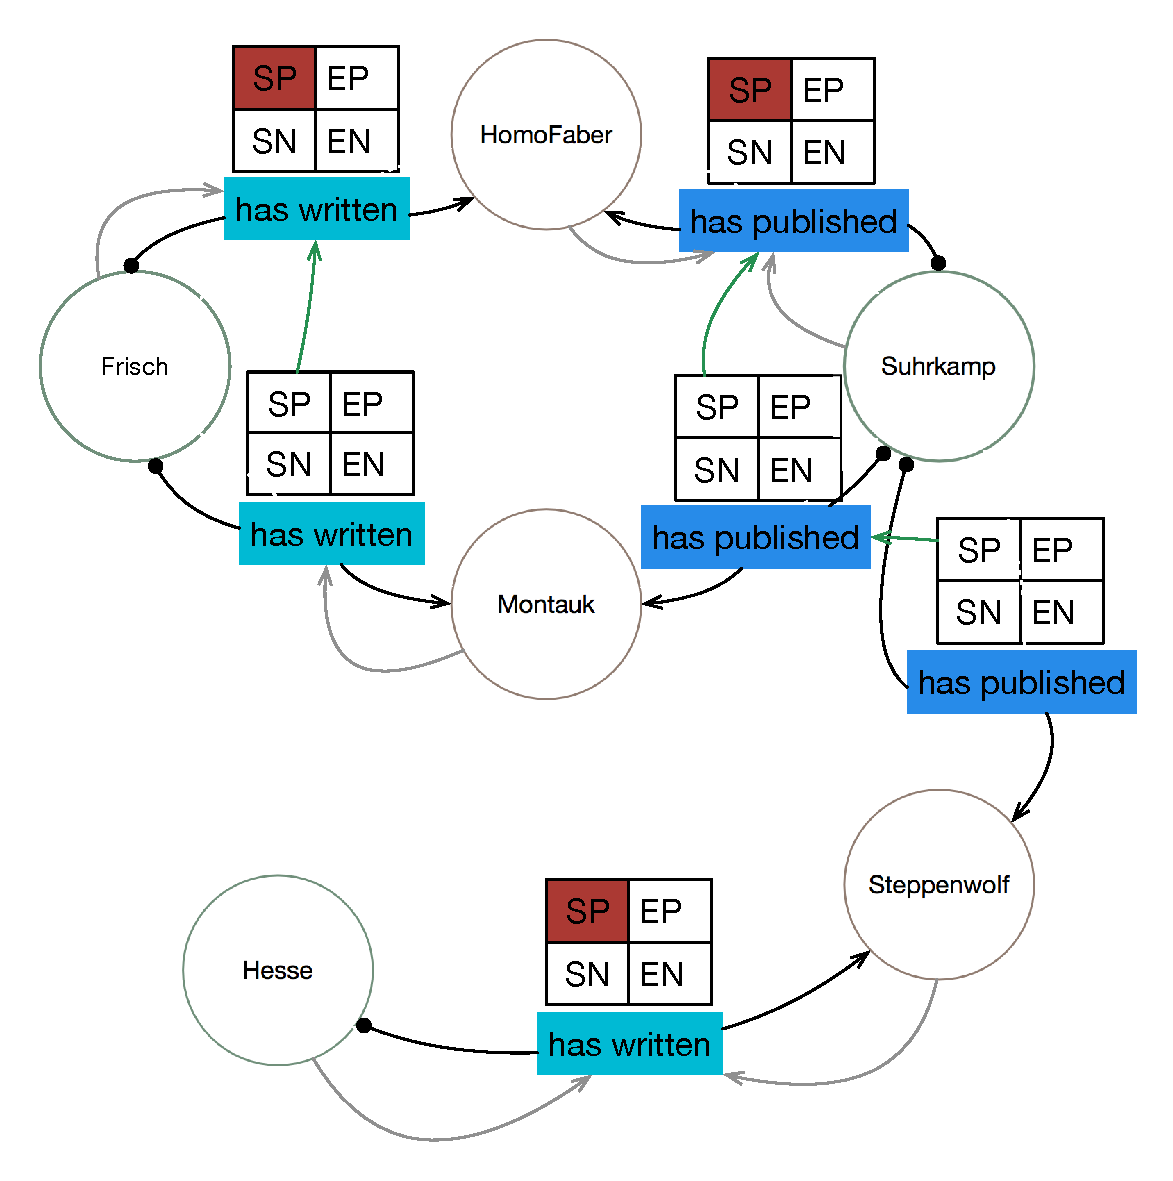
\includegraphics[width=0.9\textwidth]{images/StartNodePrevRel.eps}
	\caption{Start Node Previous Relationship}
	\label{fig5}
\end{figure}

In figure \ref{fig6} the links for the end-node previous relationship are added analogue to start-node previous relationship.

\begin{figure}
	\centering
 	 	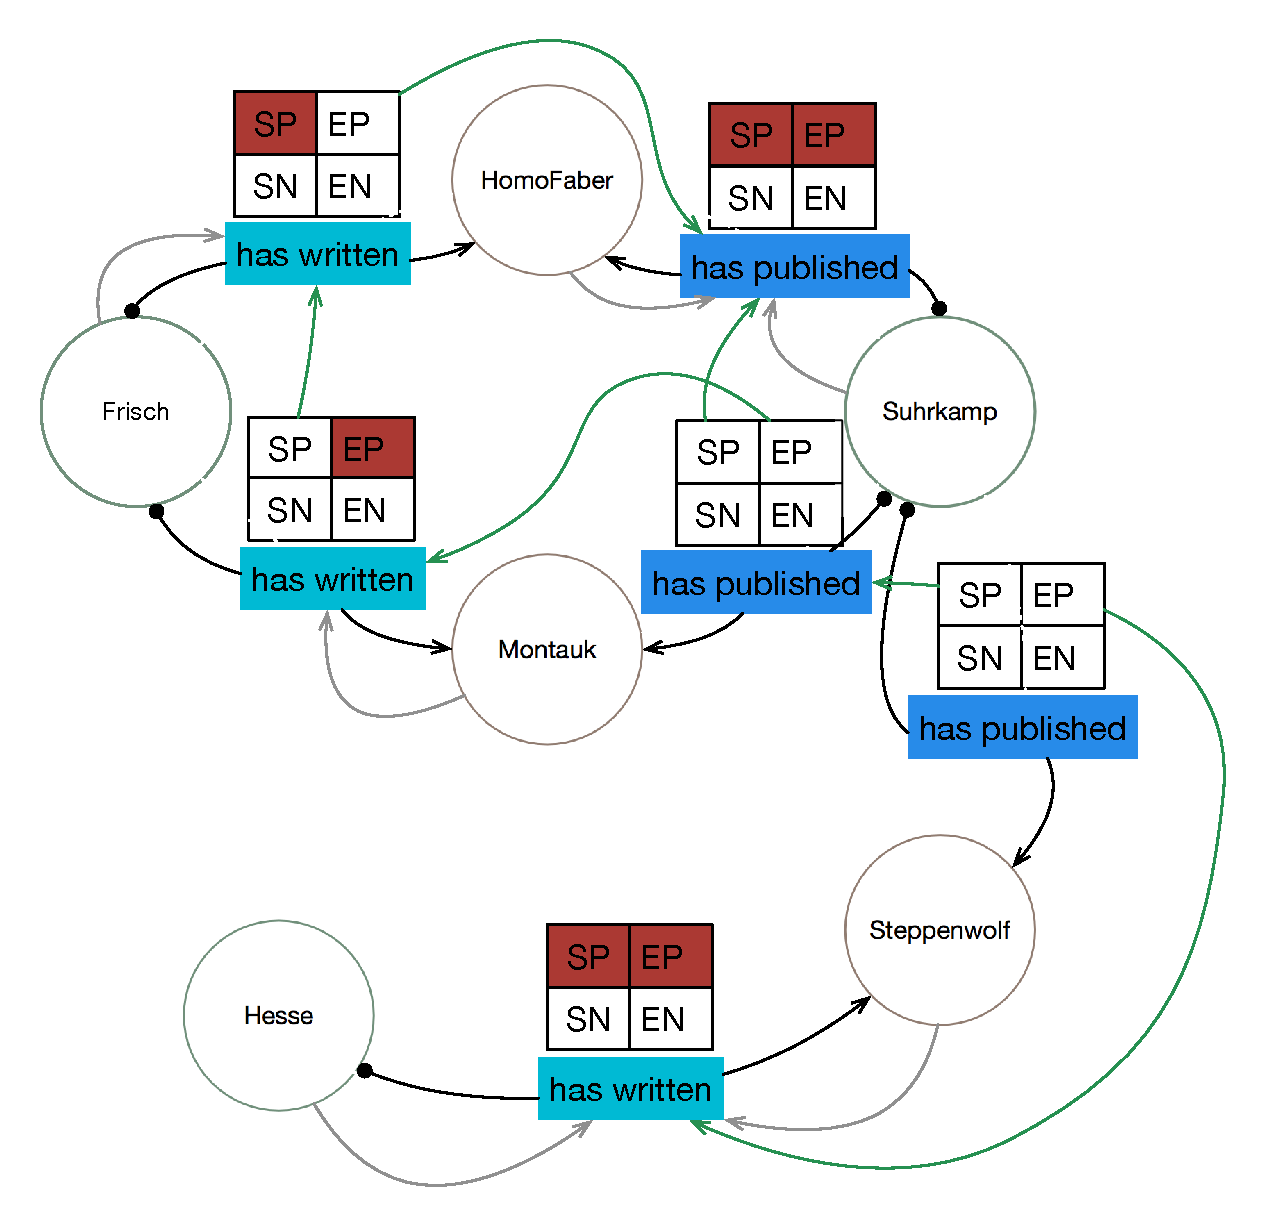
\includegraphics[width=0.9\textwidth]{images/EndNodePrevRel.eps}
	\caption{End Node Previous Relationship}
	\label{fig6}
\end{figure}

Now in figure \ref{fig7} all double linked lists are complete. This is how the graph displayed in figure \ref{fig1} would be stored. 

\begin{figure}
	\centering
 	 	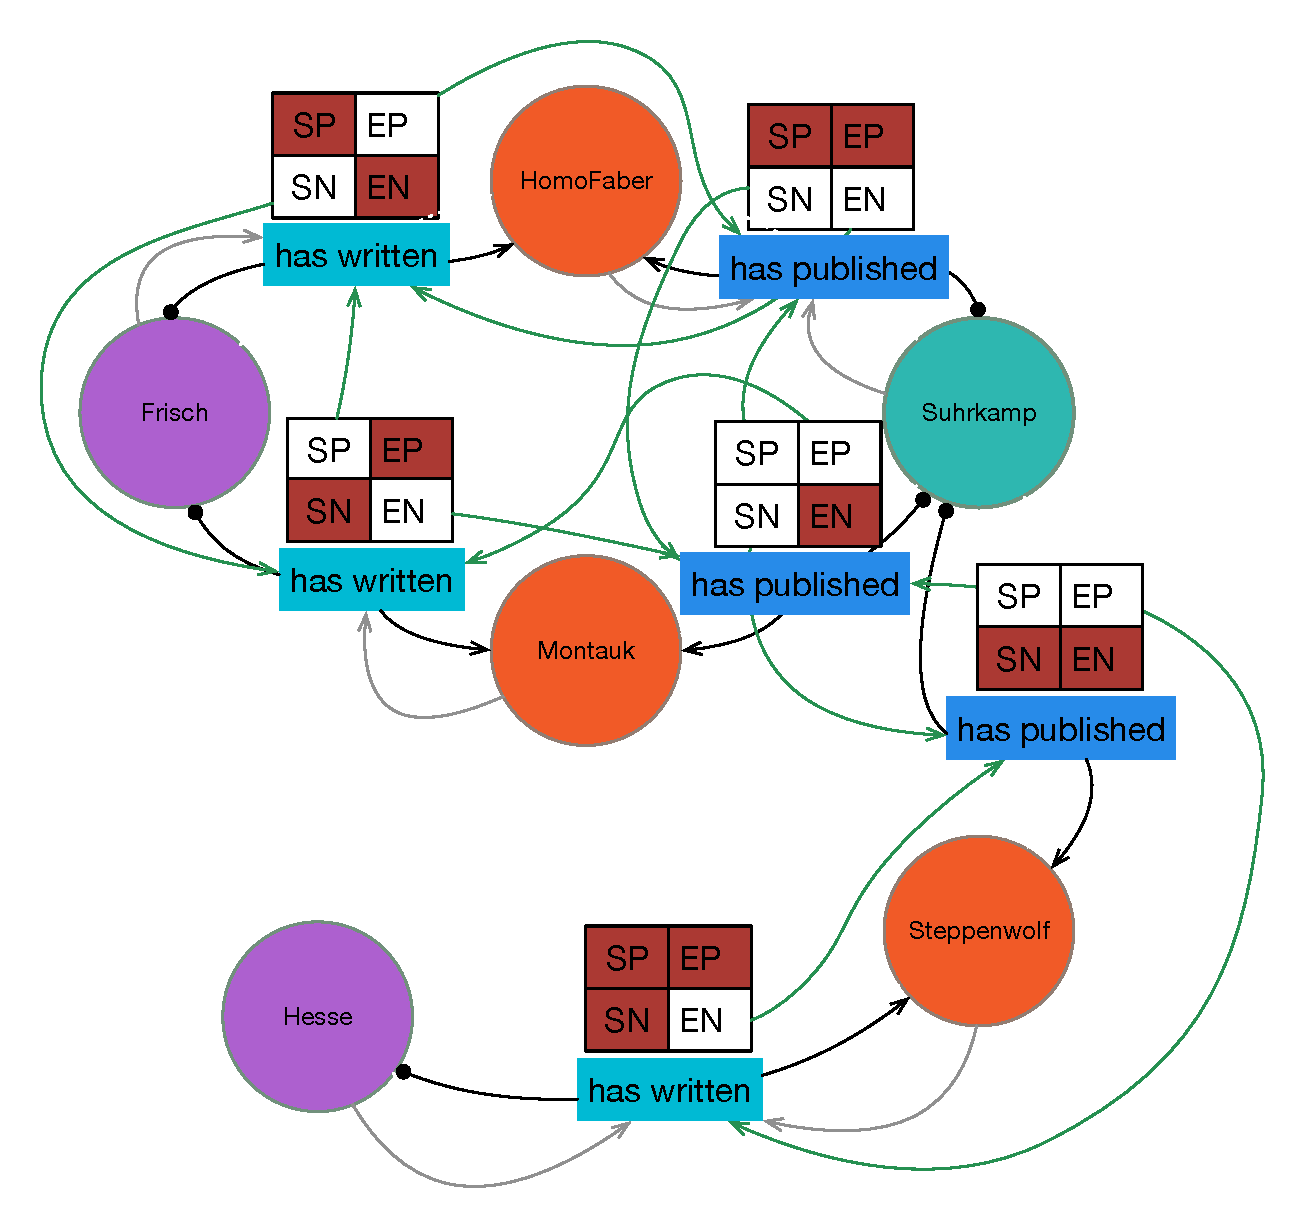
\includegraphics[width=0.9\textwidth]{images/complete.eps}
	\caption{All Pointers Displyed}
	\label{fig7}
\end{figure}

\begin{figure}
	\centering
 	 	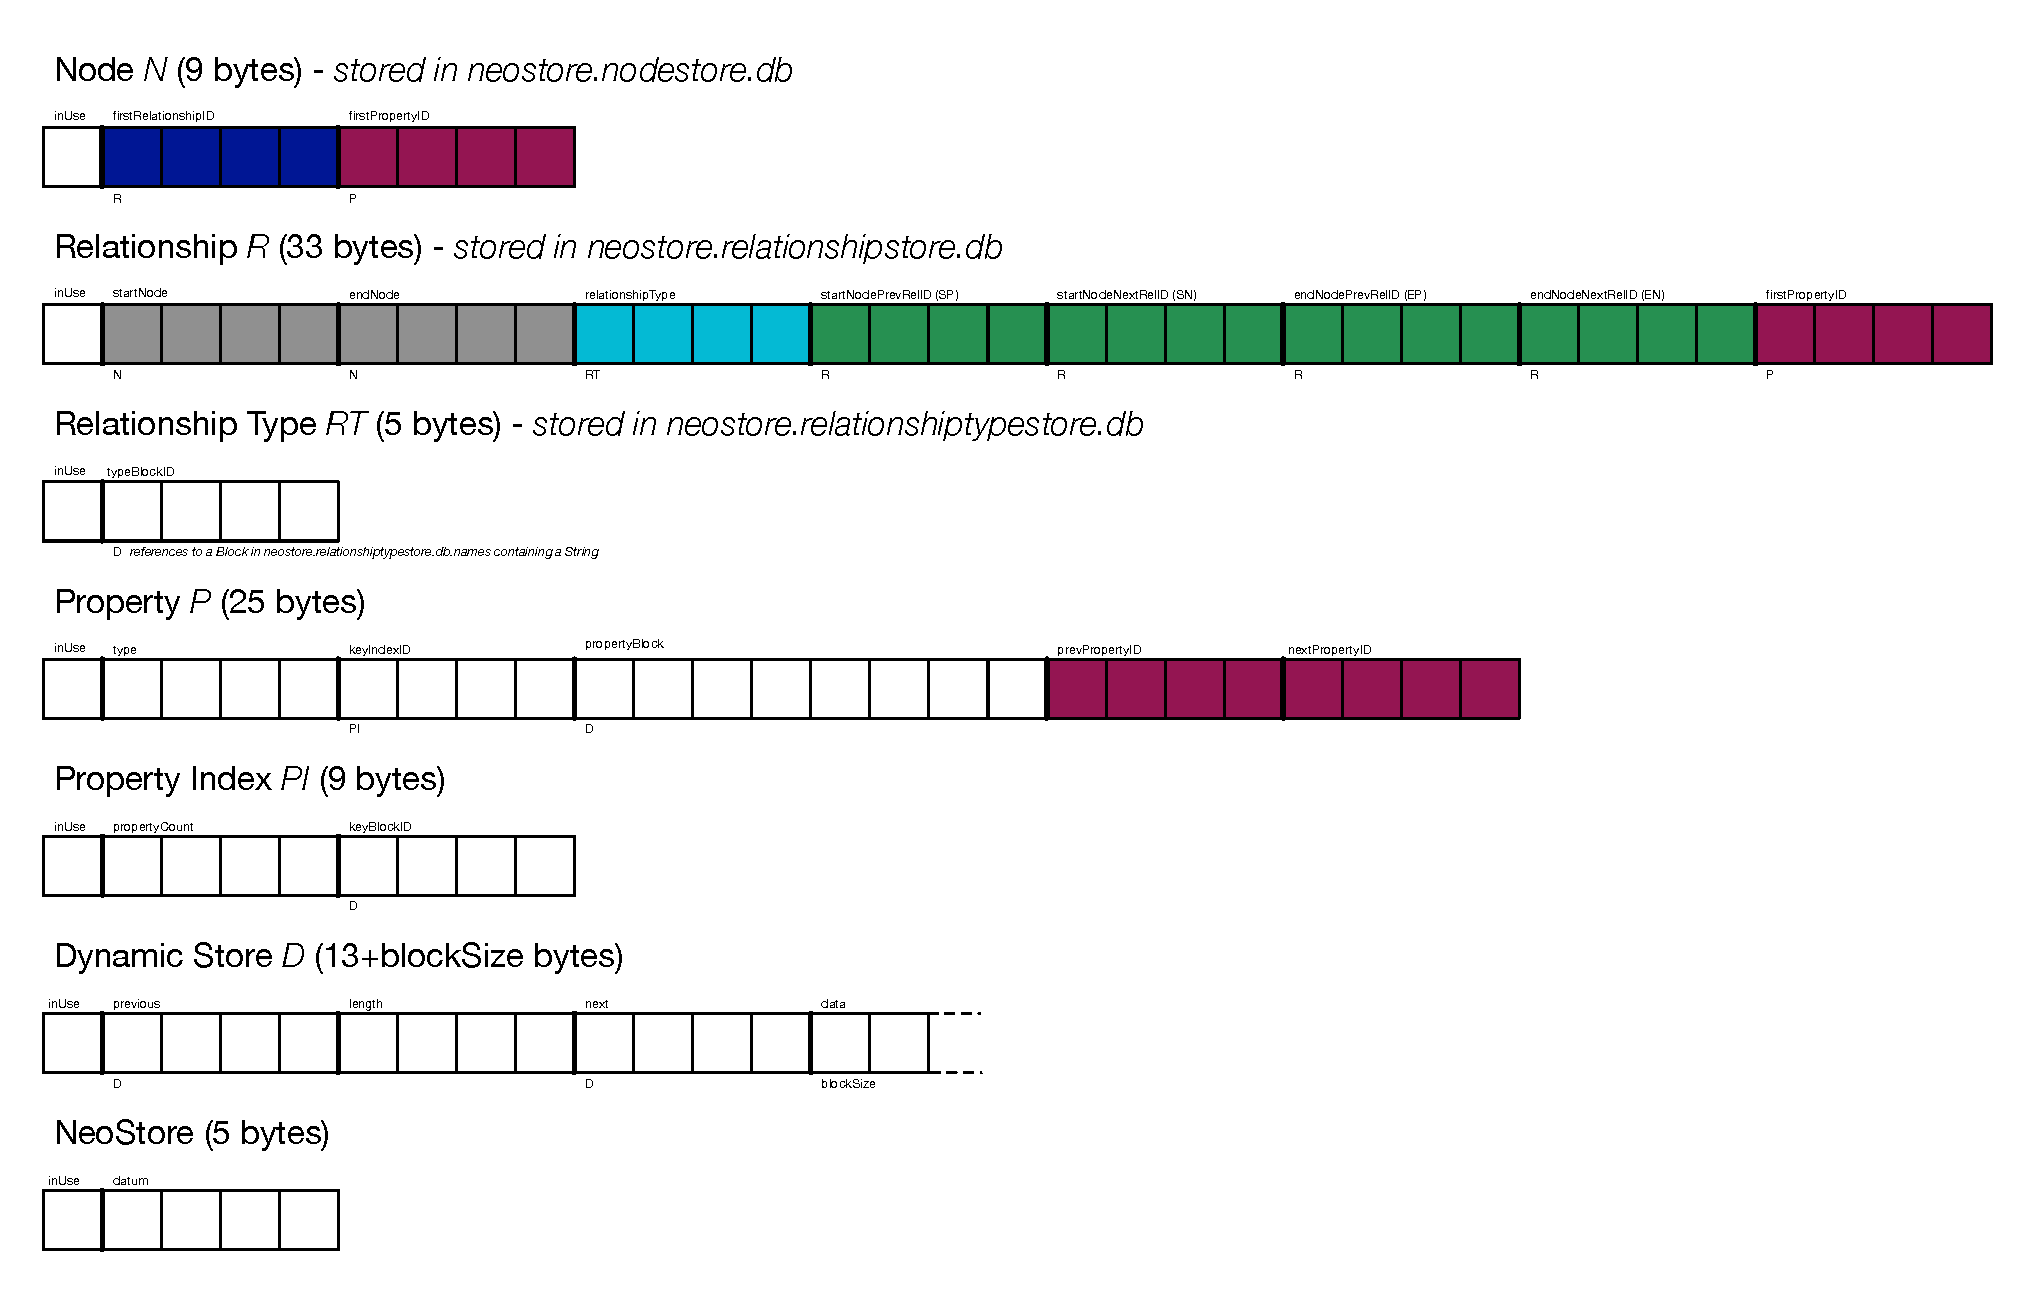
\includegraphics[width=1.2\textwidth, angle=90]{images/NeoBytes.eps}
	\caption{NeoBytes}
	\label{fig8}
\end{figure}

\newpage
%!TEX root = ../neo4j.tex

\section{Neo4j in BI}

\subsection{Business Intelligence}

"Business intelligence (BI) is a term that refers to ideas, practices and technologies for turning raw data into information that businesses can use to make better organizational decisions. Businesses that employ Bi effectively can transform information into growth by gaining a clear understanding of their strength and weaknesses, cutting costs and losses, streamlining internal processes and increasing revenue." \cite{neo4jBIDef:2014}. \nocite{BiSlides:2013}

\subsection{Why are graph databases good for BI?}

Graphs can easily visualize data based on how it exists in reality. This is shown in our book example. There are no complexe transformations needed in order to store information.
The more data a company gathers the more complex it gets to model the information in order to use it. This is the cause of the fact that data usually is inherently hierarchical and/or connected. BI relates on the useage of large amounts of data but still misses performance when it comes to "transform information into growth" \cite{neo4jBIDef:2014}. Business demands are increasing with the amount of customers and therefore the amount of data and because of the usual deep diving hierarchical structures of regular SQL databases the results are long searching times as well as complexe search queries. As we all know IT is a real time business. No bank transfer can wait minutes or seconds for its closure. User expectations are growing and there have to be new alternatives to store data. Graph databases are an entrenched solution to this problem, Neo4j is the market standard and a few steps ahead of others because it stores data in a real graph.

\subsection{BI and graph databases}

Graph databases can, like any other type of database be used in many applications of interest. One of them is Business Intelligence. With the help of analytical queries data can be "naturally expressed via an OLAP-like aggregation framework" \cite{BI:2013}. By using simple graph theory like weighted edges, productions lines as well as the shipment of products from the producer to the customer can easily be mapped into a graph database. From there on factors like location, storing, capacity etc. can be analyzed for instance to minimize waiting times of the product at different stages of the delivery or to spot the fastest and slowest routes from one location to another. Because of the size of data grouping and aggregation is required in order to pre-computate information within the database in form of materialized views containing frequently asked aggregates. This pre-processing enables the use of datawarehouses and more analytical processing on the data, also with the regard on more dimension \cite{views}.

\newpage
\printbibliography

\end{document}